\documentclass[11pt,a4paper]{article}
\usepackage[margin=2.3cm]{geometry}
\usepackage{graphicx,booktabs,amsmath,amssymb,caption,subcaption,tabularx}
\usepackage[table]{xcolor}
\usepackage[hidelinks]{hyperref}
\usepackage{microtype}
\captionsetup{font=small,labelfont=bf}
\setlength{\parskip}{2pt}
% Figures: put new ones in report/figures/. Ky's existing figures are found automatically.
\graphicspath{{figures/}{../SC4020-Ky/figures/}}

% ---------------------------------------------------------------
% Team macros. Set \draftfalse before submission: owners, TODOs and
% DECIDE notes then disappear from the PDF.
\newif\ifdraft \drafttrue
\ifdraft
  \newcommand{\owner}[1]{\par\noindent{\small\color{gray}Owner: #1}\par\smallskip}
  \newcommand{\todo}[2]{{\color{red}[\textbf{#1}: #2]}}
  \newcommand{\decide}[1]{{\color{blue}[\textbf{DECIDE}: #1]}}
  \newcommand{\figtodo}[2]{\fbox{\parbox[c][2.6cm][c]{0.92\linewidth}{\centering\small\color{red}\textbf{#1}: #2}}}
\else
  \newcommand{\owner}[1]{}
  \newcommand{\todo}[2]{}
  \newcommand{\decide}[1]{}
  \newcommand{\figtodo}[2]{}
\fi
% ---------------------------------------------------------------

\title{\vspace{-1.2cm}\textbf{When Does Density Beat Centroids?\\
A Comparative Study of Clustering Methods Across Data Geometries}\\[2pt]
\normalsize\decide{final title}}
\author{SC4020 Project 1 --- Group XX\\
\small\todo{All}{full names exactly as on student cards; replace XX with group ID}}
\date{}

\begin{document}
\maketitle
\vspace{-0.9cm}

% Owner: Ky. Write LAST, after Section 3 numbers are final.
\begin{abstract}
\noindent
\owner{Ky (write last)}
% [Ky]: draft (about 230 words) following the thesis proposed below; revise once the title is decided.
Clustering methods differ in what they take a cluster to be, and real data break those ideas in
different ways. We compare K-means, K-means++, DBSCAN and HDBSCAN on eight datasets, each chosen to test
one data property: curved shapes, long belts of uneven density, density contrast within a city, rare
classes, high dimensions, classes of unequal spread, and data with no gaps between groups. We ask where
each method fails, whether the scores available without labels reveal those failures, and whether known
remedies repair them. Each method failed where the data broke its idea of a cluster. K-means cut the
curved classes of make\_moons (ARI 0.48 against 0.98 for DBSCAN); one DBSCAN radius clustered 90\% of
earthquakes in the dense south-west Pacific but 20\% in the Americas; and in 7 to 50 dimensions the
density methods fell to ARI 0.03 to 0.05. The silhouette did not reveal these failures: on five of six
labelled datasets the method with the top silhouette was not the one that matched the labels best, and
on Ecoli it ranked the four methods almost in reverse (Spearman $\rho=-0.80$). Rerunning each result on
fake data caught methods that found nothing real, but not ones that found the wrong structure. Surface
distance, HDBSCAN and standardisation each fixed a specific failure at a cost; none produced clusters in
data with no gaps. The choice of method should follow from the structure of the data, and every score
needs a check against fake data.


\decide{Thesis, proposed 7 Oct (Wei Yew), to match the research question in Section~\ref{sec:intro}:
each method fails where the data break its idea of a cluster (RQ1); the silhouette does not reveal
these failures, a fake-data check reveals only some, and the rest need checks aimed at a known problem
(RQ2); known remedies fix some failures at a cost, and none fixes data with no gaps (RQ3).}
\end{abstract}

\section{Introduction}\label{sec:intro}
\owner{Wei Yew (draft); Ky to review}

\subsection{Motivation}
Clustering is used where no answer key exists. A seismologist grouping earthquake epicentres wants
active fault systems; a housing analyst grouping resale transactions wants market segments. Neither
has labels to check a result against.

Each clustering method carries its own idea of what a cluster is. K-means~\cite{lloyd1982} looks for
compact groups around a centre and assigns every point to one of them. DBSCAN~\cite{ester1996} and
HDBSCAN~\cite{campello2013} look for dense regions separated by sparse space, and leave points in the
sparse space as noise. Whether or not that idea matches the data, the method returns a partition. On
one year of global earthquakes, K-means returns six tidy regions, one of which joins five plate
boundaries lying 2{,}932 to 11{,}449\,km apart (Section~\ref{sec:shape}). Nothing in the output says
that this has happened. An analyst without labels usually judges the result by an internal score such
as the silhouette~\cite{rousseeuw1987}, which rates how compact and well separated the clusters are,
and that score is itself built on the K-means idea of a cluster.

\subsection{Research question}
This report asks one question: \emph{when a clustering method's idea of a cluster does not match the
data, does it fail, and can the failure be detected without labels?} We split it into three parts.
\begin{description}\itemsep1pt
\item[RQ1, cause.] Which property of the data breaks which method? We consider cluster shape, density
that varies between clusters, the number of dimensions, the absence of gaps between groups, feature
scale, and values recorded in steps.
\item[RQ2, detection.] Do checks that need no labels reveal those failures? We test the silhouette, the
Davies--Bouldin index, the share of points labelled noise, and a fake-data check: the same method run
on data whose features have been shuffled independently, which keeps each feature's values but removes
any joint structure.
\item[RQ3, remedy.] For each failure, does a known remedy help, and what does it cost?
\end{description}

We compare four methods, K-means with random starts, K-means++~\cite{arthur2007}, DBSCAN and HDBSCAN,
on eight datasets (Table~\ref{tab:data}). Each dataset was chosen to test one data property, most of
them a property that breaks at least one method's assumption. Six have class labels, so a method's output can be scored against them with the
Adjusted Rand Index (ARI)~\cite{hubert1985}, and the internal scores can be checked against that
answer. Two have no labels (earthquakes, Uber pickups); there we judge failures on maps, against known
geography.
Gaussian mixtures, spectral clustering and agglomerative clustering appear only as reference points on
the labelled datasets where we ran them (D1, D5, D6, D7), not as part of the main comparison.

\subsection{Findings in brief}
% Sources: lam/results/{make_moons,fashion_mnist,wine}_results.csv; hoanganh/results/breast_cancer_results.csv;
% SC4020-Ky/data/raw/main.csv (Ecoli); weiyew/sc4020-earthquake/results/{case_density_regions,
% method_comparison,ablation_distance}.csv; weiyew/sc4020-hdb/results/comparison.csv.
% RQ2 count, method with top silhouette vs method with top ARI, density settings within the 50% noise cap:
% D1 K-means 0.495 (ARI 0.481) vs Spectral 1.000; D4 HDBSCAN 0.483 (0.339) vs K-Means++ 0.731;
% D5 K-means 0.202 (0.343) vs Spectral 0.398; D6 HDBSCAN 0.359 (0.263) vs K-means 0.897;
% D7 K-means 0.343 (0.654) vs GMM 0.774; D8 K-means is top on both (not counted).
\begin{description}\itemsep1pt
\item[RQ1.] Each method failed where the data broke its assumption. K-means split the two interleaved
half-moons of D1 wrongly (ARI 0.48) and merged distant belts on D2. With one radius, DBSCAN clustered
90\% of earthquakes in the dense south-west Pacific but only 20\% in the sparser Americas. In 50
dimensions (D5) it barely matched the labels (ARI 0.03). On D8, where housing sales form one mass with no
gaps, both density methods returned one dominant cluster.
\item[RQ2.] The silhouette did not reveal these failures. On five of the six labelled datasets, the
method with the highest silhouette was not the one that matched the labels best. On D1 it ranks K-means
first (0.495 against 0.392 for DBSCAN), although DBSCAN recovers the moons (ARI 0.98 against 0.48). On
Ecoli (D4) it orders the four methods almost exactly opposite to ARI (Spearman $\rho=-0.80$). The
fake-data check, which we ran on D2 and D8, does better, but only partly. It detects when a method finds nothing real: on D8 both
density methods score below the same setting on shuffled data. It does not detect the wrong structure:
on D2, K-means scores well above shuffled coordinates (silhouette 0.528 against 0.391) while merging
unrelated belts. Two failures were found only by checks aimed at a known problem: clusters cut at the
$180^\circ$ meridian, and clusters that are just one recorded storey band.
\item[RQ3.] Known remedies repaired some failures and not others. Measuring distance on the sphere kept
all 92 close earthquake pairs across the $180^\circ$ meridian together, where flat coordinates kept
none. HDBSCAN raised the clustered share of the Americas from 20\% to 62\%, at the cost of trimming the
densest belts (78\% against 90\%). Nothing we tried produced meaningful density clusters on D8 with all
four features: capping the size of the largest cluster only made the rule select storey bands.
\end{description}
\todo{Lam, Ky, Hoang Anh}{confirm the RQ2 numbers above are your settings under the shared selection
rule (Section~\ref{sec:protocol}); the comment above lists each one.}

Section~\ref{sec:methods} describes the methods and Section~\ref{sec:experiments} the datasets,
protocol and results, grouped by data property. Section~\ref{sec:conclusion} turns them into guidance.

\subsection{Related work}
\paragraph{Centroid and mixture models.} Lloyd's algorithm~\cite{lloyd1982}
minimises the within-cluster sum of squared distances by alternating assignment and
centroid updates. It converges to a local optimum that depends on the starting
centres. K-means++~\cite{arthur2007} picks each starting centre with probability
proportional to its squared distance from the centres already chosen, which gives an
$O(\log k)$ approximation to the optimum in expectation. A Gaussian mixture fitted by
EM~\cite{dempster1977} generalises K-means to ellipsoidal clusters with soft
assignments. Agglomerative clustering builds a hierarchy by repeatedly merging the
closest pair of clusters. Under Ward's criterion~\cite{ward1963} the merge cost is the
increase in within-cluster variance, the same objective as K-means.

\paragraph{Density-based methods.} DBSCAN~\cite{ester1996} defines a cluster as a
maximal set of density-connected points. A point is a core point if at least
\texttt{minPts} points lie within radius $\varepsilon$. Points reachable from no core
point are noise. The method needs no $k$ and imposes no shape, but its single global
$\varepsilon$ assumes all clusters have similar density. OPTICS~\cite{ankerst1999}
orders points by reachability so that clusters at several densities can be read from
one plot. HDBSCAN~\cite{campello2013} builds a hierarchy over mutual reachability
distances and keeps the clusters that persist longest. This removes $\varepsilon$ and
leaves a minimum cluster size as the main parameter.

\paragraph{Graph-based methods.} Spectral clustering~\cite{ng2002} embeds the points
using the leading eigenvectors of a normalised affinity matrix, then runs K-means in
that embedding. Groups connected through the affinity graph become compact in the
embedding, so non-convex clusters can be separated. A dense affinity matrix needs
$O(n^2)$ memory, which limits the method to modest $n$.

\paragraph{Validation and cluster tendency.} Internal indices, such as the
silhouette~\cite{rousseeuw1987}, Davies--Bouldin~\cite{davies1979} and
Calinski--Harabasz~\cite{calinski1974} indices, score a partition from the data
alone. External indices such as the Adjusted Rand Index~\cite{hubert1985} compare it
with known labels. Von Luxburg et al.~\cite{luxburg2012} argue that no criterion can
judge a clustering apart from its intended use. A separate line of work tests whether
data contain clusters at all. The Hopkins statistic~\cite{hopkins1954} compares
nearest-neighbour distances in the data with those in uniformly random points. The
gap statistic~\cite{tibshirani2001} compares within-cluster dispersion with its value
on reference data drawn from a null distribution. Our fake-data check applies the
same idea to every method we compare. In high dimensions the ratio of nearest to
farthest neighbour distance tends to one~\cite{beyer1999}, which weakens any method
built on a density threshold.

\section{Methods}\label{sec:methods}
\owner{Ky (K-Means, K-Means++, DBSCAN, HDBSCAN); Lam (GMM, Spectral); Hoang Anh (Agglomerative)}

% Rubric: "clear explanation of the tasks and the methods". Each method: idea, objective or
% rule, parameters, complexity, assumption it makes, how it fails.

\subsection{K-Means and K-Means++}
% Ky. Code: SC4020-Ky/src/core.py (run_kmeans)
K-means~\cite{lloyd1982} looks for $k$ centres $\boldsymbol{\mu}_1,\dots,\boldsymbol{\mu}_k$ that minimise
the within-cluster sum of squares (inertia), $J=\sum_{i=1}^{n}\min_j\lVert\mathbf{x}_i-\boldsymbol{\mu}_j\rVert^2$.
Each iteration assigns every point to its nearest centre and moves each centre to the mean of its points.
$J$ never rises, so the method stops at a local optimum that depends on the starting centres. One
iteration costs $O(nkd)$. Random starts pick $k$ data points uniformly. K-means++~\cite{arthur2007} picks
the first centre at random and each next one with probability proportional to its squared distance from
the nearest centre already chosen. Only the start differs, so we treat the two as one method with two
initialisations (Ablation~A). We use scikit-learn's \texttt{KMeans} with 10 starts; the only parameter is
$k$. Because $J$ sums squared Euclidean distances, K-means suits compact, roughly round clusters of
similar spread. It cuts curved or elongated clusters, gives every point a cluster, so outliers pull the
centres, and depends on the scale of each feature (Ablation~C).
\subsection{DBSCAN}
% Ky. Code: SC4020-Ky/src/core.py (run_dbscan, k_distance_curve, knee)
DBSCAN~\cite{ester1996} takes a radius $\varepsilon$ and a count \texttt{minPts}. A point is a core point
if at least \texttt{minPts} points lie within $\varepsilon$ of it. Core points within $\varepsilon$ of
each other join the same cluster, points within $\varepsilon$ of a core point join its cluster as border
points, and every other point is noise. The method needs no $k$ and assumes no shape, and on coordinates
$\varepsilon$ is a distance on the ground that an analyst can judge. With a spatial index a fit costs
about $O(n\log n)$ in few dimensions, rising towards $O(n^2)$ in many dimensions or with a large
$\varepsilon$. A reference value for $\varepsilon$ comes from the k-distance curve, each point's distance
to its \texttt{minPts}-th nearest neighbour in sorted order; its knee is the point farthest from the line
joining the two ends of the curve. The weakness is the single radius. It assumes all clusters have
similar density, so a radius that separates dense clusters calls sparse ones noise, and one that keeps
sparse clusters merges dense ones. In many dimensions distances become alike~\cite{beyer1999}, and a
radius separates little.
\subsection{HDBSCAN}
% Ky. Code: SC4020-Ky/src/core.py (run_hdbscan)
HDBSCAN~\cite{campello2013} removes $\varepsilon$. Each point's core distance is the distance to its
$m$-th nearest neighbour, and the mutual reachability distance
$d_{\mathrm{mr}}(a,b)=\max\{\mathrm{core}(a),\mathrm{core}(b),d(a,b)\}$ pushes points in sparse regions
apart. A minimum spanning tree under $d_{\mathrm{mr}}$ holds the DBSCAN clusterings at every density
level at once. The tree is condensed by dropping any split that leaves fewer than
\texttt{min\_cluster\_size} points, and the clusters that persist over the widest range of density are
kept; the remaining points are noise. Different branches can thus be cut at different densities, which is
what DBSCAN cannot do. We use scikit-learn's \texttt{HDBSCAN}; the main parameter is
\texttt{min\_cluster\_size}, and $m$ (\texttt{min\_samples}) defaults to it. A fit costs between
$O(n\log n)$ and $O(n^2)$. Because \texttt{min\_cluster\_size} is a count, the result changes with the
size of the sample. HDBSCAN can call large parts of the data noise, and like DBSCAN it has nothing to
find where the data have no density gaps.
\subsection{Gaussian Mixture Model}
% Lam. Code: lam/src/sc4020/clustering.py
A Gaussian mixture model (GMM) treats the data as drawn from $k$ Gaussians,
$p(\mathbf{x})=\sum_{j=1}^{k}\pi_j\,\mathcal{N}(\mathbf{x}\mid\boldsymbol{\mu}_j,\boldsymbol{\Sigma}_j)$,
and fits the weights $\pi_j$, means and covariances by expectation--maximisation (EM)~\cite{dempster1977}.
The E-step computes each point's responsibility (posterior probability) under every component; the
M-step re-estimates $\pi_j$, $\boldsymbol{\mu}_j$ and $\boldsymbol{\Sigma}_j$ from those soft
assignments; the two steps repeat until the log-likelihood stops improving. Each point is then given
its most probable component. We use scikit-learn's \texttt{GaussianMixture}~\cite{pedregosa2011} with
\emph{full} covariance matrices (the default), $k$-means initialisation, one start and a fixed seed.
The only parameter is the number of components $k$, which we set to the number of classes on labelled
data and to the silhouette-best $k\in[2,10]$ otherwise. One EM iteration costs $O(nkd^2+kd^3)$.
GMM generalises K-Means: full covariances allow ellipsoidal clusters of different size, orientation
and weight, but each cluster must still be a single convex blob. It fails on curved or nested shapes,
has no noise label, and with full covariances it needs many points per component when $d$ is large.
\subsection{Spectral clustering}
% Lam. Code: lam/src/sc4020/clustering.py; affinity per dataset in lam/notebooks/0*_*.ipynb
Spectral clustering~\cite{ng2002} turns clustering into graph partitioning. It (i) builds an affinity
matrix $W$ whose entry $w_{ij}$ measures how similar points $i$ and $j$ are; (ii) forms the normalised
graph Laplacian and takes its $k$ leading eigenvectors, giving each point a $k$-dimensional embedding;
(iii) runs K-Means on the rows of that embedding. Points joined by a chain of close neighbours land
near each other in the embedding even when they are far apart in the input space, so the method can
recover curved and non-convex clusters. We use scikit-learn's \texttt{SpectralClustering} with two
affinities: an RBF kernel $w_{ij}=\exp(-\gamma\lVert\mathbf{x}_i-\mathbf{x}_j\rVert^2)$, $\gamma=1$,
for roughly globular data (D6 Wine, Mall), and a symmetric 10-nearest-neighbour graph for manifold-shaped
data (D1 make\_moons, D5 Fashion-MNIST), where one global bandwidth fits poorly. Parameters are $k$
and the affinity (with $\gamma$ or the neighbour count). A dense RBF affinity costs $O(n^2d)$ time and
$O(n^2)$ memory, and a full eigendecomposition $O(n^3)$; the sparse $k$-NN graph with an iterative
eigensolver is much cheaper but still limits $n$ (Section~\ref{sec:runtime}). Spectral clustering
needs $k$, has no noise label, and is sensitive to the affinity scale.
\subsection{Agglomerative clustering}
\habegin
% Source: hoanganh/src/sc4020/clustering.py (wine_models, breast_cancer_models);
% ARI from hoanganh/results/{wine,breast_cancer}_results.csv.
\hatag{}Agglomerative clustering starts with every point as its own cluster and repeatedly merges the two
closest clusters until $k$ remain. The linkage defines which two are closest. We use Ward
linkage~\cite{ward1963}, which merges the pair whose union raises the total within-cluster variance
least. This is the K-means objective, searched greedily from the bottom up. The method therefore
needs no starting centres and returns the same partition on every run, which makes it a direct check
on K-means: same objective, different search. The only parameter is $k$, set to the number of classes
(3 on D6, 2 on D7); distances are Euclidean on standardised features. It needs $O(n^2)$ time and
memory for the pairwise distances, so we ran it on the two small tables only ($n=178$ and $n=569$).
Like K-means, it assumes compact clusters, assigns every point and has no noise label. Its own
weakness is that a merge is never undone, so an early mistake stays in the final partition. On both
datasets it matched the labels less well than K-means (ARI 0.790 against 0.897 on D6, 0.575 against
0.654 on D7).
\haend

\begin{table}[h]\centering\small
\caption{Structural assumptions of the methods compared.}
\label{tab:assump}
\resizebox{\textwidth}{!}{\begin{tabular}{lccccccc}
\toprule
& \textbf{K-Means} & \textbf{K-Means++} & \textbf{DBSCAN} & \textbf{HDBSCAN}
& \textbf{GMM} & \textbf{Spectral} & \hatag\textbf{Agglom.} \\
\midrule
Cluster shape assumed      & isotropic & isotropic & arbitrary & arbitrary & ellipsoidal & connected (graph) & compact (Ward) \\
Requires $k$               & yes & yes & no & no & yes & yes & yes \\
Explicit noise label       & no & no & yes & yes & no & no & no \\
Handles varying density    & no & no & no & yes & partly\textsuperscript{b} & partly\textsuperscript{c} & no \\
Parameter is interpretable & no & no & yes (km) & partly & no & no & no \\
Time complexity            & $O(nkdi)$ & $O(nkdi)$ & $O(n\log n)$\textsuperscript{a} & $O(n\log n)$\textsuperscript{a} & $O(nkd^2 i)$ & $O(n^2d+n^3)$\textsuperscript{d} & $O(n^2)$ \\
\bottomrule
\end{tabular}}
\par\raggedright\footnotesize\textsuperscript{a}\,With an effective spatial index; $O(n^2)$ worst case.
\textsuperscript{b}\,Per-component covariance and weight.
\textsuperscript{c}\,With a $k$-NN affinity, which adapts to local scale.
\textsuperscript{d}\,Dense RBF affinity and full eigendecomposition; lower with a sparse $k$-NN graph.
\end{table}


\section{Experiments}\label{sec:experiments}
\subsection{Datasets}\label{sec:data}
\owner{each dataset's owner writes its paragraph (max.\ 120 words)}

% Rubric: "target challenging datasets". Say why each dataset is hard for at least one method.

\begin{table}[h]\centering\small
\caption{Datasets, grouped by the data property each one tests. \decide{final list; drop or keep Mall;
Ky's 1965--2016 earthquakes replaced by the 2023 surface-distance pipeline?}}
\label{tab:data}
\resizebox{\textwidth}{!}{\begin{tabular}{lllrrll}
\toprule
\textbf{ID} & \textbf{Dataset} & \textbf{Owner} & \textbf{$n$} & \textbf{$d$} & \textbf{Labels} & \textbf{Property tested} \\
\midrule
D1 & make\_moons (synthetic)          & Lam            & 1{,}000  & 2        & 2 classes    & curved shapes (control) \\
D2 & Earthquakes, 2023, M$\geq$4.5    & Wei Yew        & 7{,}643  & 2        & none         & long belts, uneven density \\
D3 & Uber NYC pickups, Apr 2014       & Ky, Hoang Anh  & \decide{6k or 15k} & 2 & none      & density contrast in a city \\
D4 & Ecoli                            & Ky             & 336      & 7        & 8 classes    & dimensionality, rare classes \\
D5 & Fashion-MNIST (PCA)              & Lam            & 3{,}000  & 50       & 10 classes   & high dimensions \\
D6 & Wine                             & Lam, Hoang Anh & 178      & 13       & 3 classes    & silhouette vs labels \\
D7 & Breast cancer (Wisconsin)        & Hoang Anh      & 569      & 30       & 2 classes    & silhouette vs labels \\
D8 & HDB resale flats, 2017--2026     & Wei Yew        & 20{,}000\textsuperscript{b} & 4 & flat type (7) & no gaps, scale, recorded ties \\
\bottomrule
\end{tabular}}
\par\raggedright\footnotesize\textsuperscript{b}\,Random sample of 234{,}294 usable sales; all 234{,}294 used for runtime (Section~\ref{sec:runtime}).
\end{table}

\paragraph{D1 make\_moons.} \todo{Lam}{generator settings (noise 0.07), why it is the shape control.}
\paragraph{D2 Earthquakes.}
% Source: weiyew/sc4020-earthquake/notebooks/eda.ipynb, sections 1, 4, 8 and 12.
Every event of magnitude 4.5 or more in 2023 from the USGS ComCat catalogue~\cite{usgs2017}: 7{,}651 events, of which
8 volcanic eruptions near Saipan are removed, leaving 7{,}643 earthquakes. We cluster the epicentre only.
Depth is left out because 44.2\% of events carry the default depth of 10\,km. Each method meets a
different difficulty. Earthquakes lie along narrow belts thousands of kilometres long, which breaks the
compact-cluster assumption of K-means. Density varies widely: the distance to the nearest earthquake
runs from 1.2\,km (5th percentile) to 100.5\,km (95th), so no single DBSCAN radius suits every belt.
And 17.2\% of earthquakes lie within $10^\circ$ of the $180^\circ$ meridian, where flat coordinates
cut the map. There are no labels.
\paragraph{D3 Uber NYC.} \todo{Ky + Hoang Anh}{one merged paragraph; agree sample size and bounding box.}
\paragraph{D4 Ecoli.} \todo{Ky}{Port from Sec.~4.1.}
\paragraph{D5 Fashion-MNIST.} \todo{Lam}{3{,}000-image sample, PCA to 50 dims; why subsampled.}
\paragraph{D6 Wine.} \todo{Lam + Hoang Anh}{one merged paragraph; both runs give K-Means ARI 0.897.}
\paragraph{D7 Breast cancer.} \todo{Hoang Anh}{30 features, standardised; benign vs malignant.}
\paragraph{D8 HDB resale.}
% Source: weiyew/sc4020-hdb/notebooks/eda.ipynb, sections 6, 10, 11 and 17;
% sample size: weiyew/sc4020-hdb/notebooks/clustering.ipynb, section 1;
% floor-area ARI: weiyew/sc4020-hdb/results/screening_labels.csv.
Every resale of a public housing flat in Singapore from January 2017, from data.gov.sg~\cite{hdb2026}. The 6{,}051
sales after June 2026 (2.5\%) have no price index value yet and are dropped, leaving 234{,}294. Methods
are compared on a random sample of 20{,}000 (seed 0); all 234{,}294 are used for runtime. There are four
features: floor area, remaining lease, storey, and price adjusted to 2026 levels with the HDB resale
price index. Flat type (7 classes) is held out as a label, but it is nearly a function of size: floor
area alone reaches ARI 0.601 against it. The data are hard for density methods. There are no gaps
between groups of flats, and storeys are recorded in 3-storey bands, so 77.7\% of sales share their
floor area, lease and storey with at least one other sale.

\subsection{Preprocessing}\label{sec:prep}
\owner{Wei Yew}
Three rules apply wherever a dataset has the property they address. Each is tested by an ablation in
Section~\ref{sec:ablation}.

\paragraph{Coordinates on the sphere.}
% Source: weiyew/sc4020-earthquake/notebooks/eda.ipynb, section 12.
Latitude and longitude treated as flat numbers put two earthquakes 6.07\,km apart at $359.94^\circ$ of
longitude from each other, because they lie on either side of the $180^\circ$ meridian. Density methods
therefore use the haversine (great-circle) distance on coordinates in radians. K-means needs a vector
space to average in, so each epicentre becomes a 3D point on the unit sphere. The straight-line distance
between two such points grows with their great-circle distance, so the clustering follows surface distance
(Ablation~B).

\paragraph{Standardised features.}
% Source: weiyew/sc4020-hdb/notebooks/eda.ipynb, section 9.
Features in their raw units are not comparable. On D8, price (in dollars) accounts for 100.0\% of the
squared distance between sales, so the other three features are ignored. Every feature is scaled to mean
0 and standard deviation 1 (Ablation~C).

\paragraph{Values recorded in steps.}
% Source: weiyew/sc4020-hdb/hdb/features.py, jitter_ties.
When a feature is recorded in steps, many points share exact values, and density methods read each shared
value as a dense spot. Before running a density method on D8, each stepped value is moved by a uniform
random amount of up to half its step: $\pm1.5$ storeys, $\pm0.5$\,m$^2$ of floor area and
$\pm\frac{1}{24}$ year of lease. Price is continuous and is left unchanged. Results are reported with and
without this jitter (Ablation~E).

\subsection{Evaluation metrics and parameter selection}\label{sec:protocol}
\owner{Ky, Wei Yew}

% Rubric: "analyze and discuss the parameter settings".

\paragraph{Metrics.}
\todo{Ky + Wei Yew}{Internal: silhouette, Davies--Bouldin, Calinski--Harabasz (noise excluded).
Coverage: noise \%, largest-cluster \%. External (labelled data): ARI, NMI (noise kept as a label).
Fake-data check: same method on shuffled columns (tabular) or uniform points (coordinates);
a result counts only if the real data scores clearly higher. Runtime.}

\paragraph{Selection rule.}
\decide{One rule for every dataset and method. Ky: $\geq3$ clusters, $\leq40\%$ noise.
Wei Yew: $\geq2$ clusters, $\leq50\%$ noise. Add a largest-cluster cap? (It picks storey-band
artefacts on HDB, Section~\ref{sec:ablation}.)}
\todo{All}{Labelled datasets: report both the rule's choice and the best-ARI (oracle) choice,
so the gap between them is visible.}

\paragraph{Parameter grids.}
% Lam: lam/src/sc4020/hyperparams.py
GMM and Spectral (Lam): $k$ set to the number of classes on labelled data, else the silhouette-best
K-Means++ $k\in[2,10]$; GMM full covariance; spectral affinity RBF ($\gamma=1$) for D6 and Mall,
10-nearest-neighbour graph for D1 and D5. Lam's DBSCAN and HDBSCAN runs: \texttt{minPts} from
$\{\lfloor m/2\rfloor, m, 2m\}$ with $m=\mathrm{clip}(2d,4,20)$, $\varepsilon$ from $\{0.5,0.75,1,1.5,2\}\times$
the k-distance knee; \texttt{min\_cluster\_size} from $\{5,10,20,30,50,n/20\}$; the setting with the
best silhouette (noise excluded, $\geq2$ clusters, $\leq50\%$ noise) is kept.
\todo{All}{One line per method: $k$ range; $\varepsilon$ grid (k-distance knee or quantiles);
\texttt{minPts}; \texttt{min\_cluster\_size} and \texttt{min\_samples}; GMM components;
spectral affinity.}

\paragraph{Reproducibility.}
\decide{shared code: Ky's src/core.py or Wei Yew's metrics.py, so every table has the same columns.}
\todo{All}{scikit-learn version, seeds, hardware.}

\subsection{Comparison by data property}\label{sec:comparison}
\owner{All}

% Rubric: "compare the performance", "strengths and weaknesses", "insightful comparisons".
% Every number must come from a results CSV in the repo. Put the path in a % comment.

\todo{All}{One results table per property (rows: dataset $\times$ method; columns: \#clusters,
noise, S, DB, ARI, NMI, time, fake-data gap). Bold the best per dataset.}

% [Wei Yew]: Table tab:cmp_d2d8 uses the shared columns; merge its rows into the per-property tables
% once the other datasets are in the same format.
% Sources: weiyew/sc4020-earthquake/results/method_comparison.csv; weiyew/sc4020-hdb/results/comparison.csv.
\begin{table}[h]\centering\small
\caption{D2 and D8 at the settings chosen in Section~\ref{sec:protocol}. S: silhouette; DB:
Davies--Bouldin; null S: silhouette of the same setting on fake data (D2: shuffled coordinates for K-means,
uniform points for density methods; D8: shuffled columns). ``none'': no clusters formed on the fake data.
D2 has no labels.}
\label{tab:cmp_d2d8}
\resizebox{\textwidth}{!}{\begin{tabular}{llrrrrrrrrr}
\toprule
\textbf{Data} & \textbf{Method} & \textbf{Clusters} & \textbf{Noise} & \textbf{Largest} & \textbf{S} & \textbf{DB}
& \textbf{ARI} & \textbf{NMI} & \textbf{Time (s)} & \textbf{Null S} \\
\midrule
D2 & K-Means ($K=6$)      & 6  & 0\%    & 44.3\% & 0.525 & 0.800 & -- & -- & 0.004 & 0.389 \\
D2 & K-Means++ ($K=6$)    & 6  & 0\%    & 31.0\% & 0.528 & 0.738 & -- & -- & 0.005 & 0.391 \\
D2 & DBSCAN (101.8\,km, 20) & 41 & 40.4\% & 11.8\% & 0.703 & 0.351 & -- & -- & 0.051 & none \\
D2 & HDBSCAN (50)         & 28 & 30.7\% & 7.5\%  & 0.757 & 0.329 & -- & -- & 1.081 & 0.320 \\
\midrule
D8 & K-Means ($K=4$)      & 4  & 0\%    & 36.2\% & 0.317 & 1.116 & 0.220 & 0.299 & 0.011 & 0.195 \\
D8 & K-Means++ ($K=4$)    & 4  & 0\%    & 35.1\% & 0.317 & 1.116 & 0.213 & 0.293 & 0.010 & 0.218 \\
D8 & DBSCAN (0.567, 10)   & 3  & 1.4\%  & 97.1\% & 0.239 & 0.732 & 0.030 & 0.091 & 0.428 & 0.330 \\
D8 & HDBSCAN (200)        & 2  & 28.5\% & 68.6\% & 0.160 & 1.133 & 0.072 & 0.101 & 2.022 & 0.593 \\
\bottomrule
\end{tabular}}
\end{table}

\subsubsection{Curved and elongated clusters}\label{sec:shape}
\owner{Lam (D1), Wei Yew (D2)}
\todo{Lam}{D1: DBSCAN ARI 0.982, Spectral 1.000, K-Means++ 0.481 (\nolinkurl{lam/results/make_moons_results.csv}).}

% Source: weiyew/sc4020-earthquake/notebooks/ablation.ipynb, section 5 (K-means belt case, printed
% centre distances); figure from the same cell.
K-means assumes compact clusters, and D2 breaks that assumption at planetary scale. Earthquakes follow
plate boundaries, so a cluster is a long,
narrow belt rather than a ball around a centre. K-Means++ with $K=6$ must cover the whole globe with six
roughly round regions, so each region takes in several unrelated belts
(Figure~\ref{fig:kmeans_belts}). One cluster of 905 earthquakes joins Turkey, the Reykjanes Ridge and
Iceland, Afghanistan and Tajikistan, Somalia and Eritrea, and the Mid-Indian Ridge. HDBSCAN finds each of
these as its own cluster, and their centres are 2{,}932 to 11{,}449\,km apart. K-means also has no noise
label, so every isolated earthquake in the oceans is assigned to some region. Its silhouette is still
0.528, well above the 0.391 of shuffled coordinates: the score confirms that the data are not random, not
that the clusters are meaningful.

\begin{figure}[h]\centering
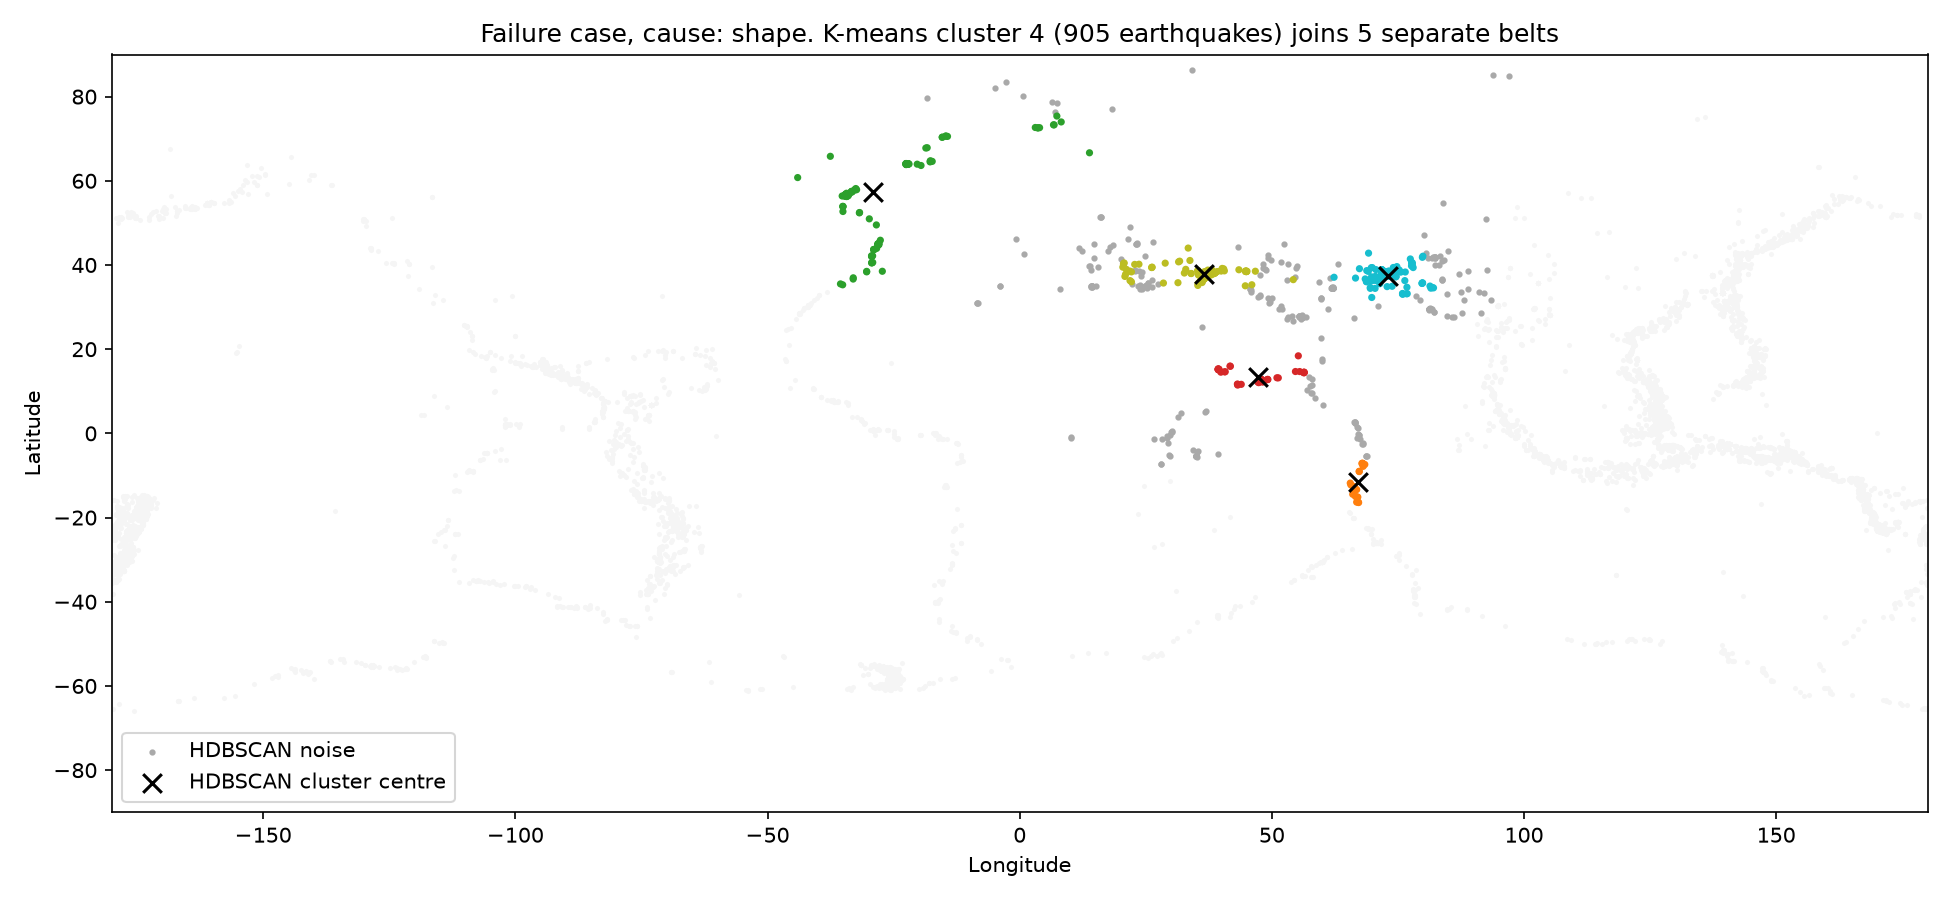
\includegraphics[width=0.9\textwidth]{eq_case_kmeans_merges_belts}
\caption{D2, failure of K-Means++ ($K=6$). All points shown in colour or dark grey belong to one K-means
cluster; colours are the HDBSCAN clusters inside it, crosses their centres. Cause: cluster shape. Belts
thousands of kilometres apart are joined because K-means can only draw compact regions.}
\label{fig:kmeans_belts}
\end{figure}

\subsubsection{Uneven density}\label{sec:density}
\owner{Wei Yew (D2), Ky and Hoang Anh (D3)}
% Sources: weiyew/sc4020-earthquake/results/case_density_regions.csv, method_comparison.csv;
% k-distance spread from weiyew/sc4020-earthquake/notebooks/eda.ipynb, section 12.
On D2 the distance to the nearest earthquake runs from 1.2\,km to 100.5\,km (5th to 95th percentile), and
the k-distance curve rises smoothly with no knee. Any single $\varepsilon$ is therefore too small for some
belts and too large for others. At the chosen $\varepsilon=101.8$\,km, DBSCAN clusters 90\% of the
earthquakes in the dense south-west Pacific but only 20\% in the sparser Americas
(Figure~\ref{fig:density}). HDBSCAN, which picks a density level per cluster, clusters 62\% of the
Americas and keeps the Mexico to Panama belt and the Chile and Argentina belt as long clusters. The price is paid in the dense
region, where it clusters 78\% instead of 90\%. Overall HDBSCAN keeps more earthquakes (69.3\% against
59.6\%) with a higher silhouette (0.757 against 0.703, Table~\ref{tab:cmp_d2d8}).

\begin{figure}[h]\centering
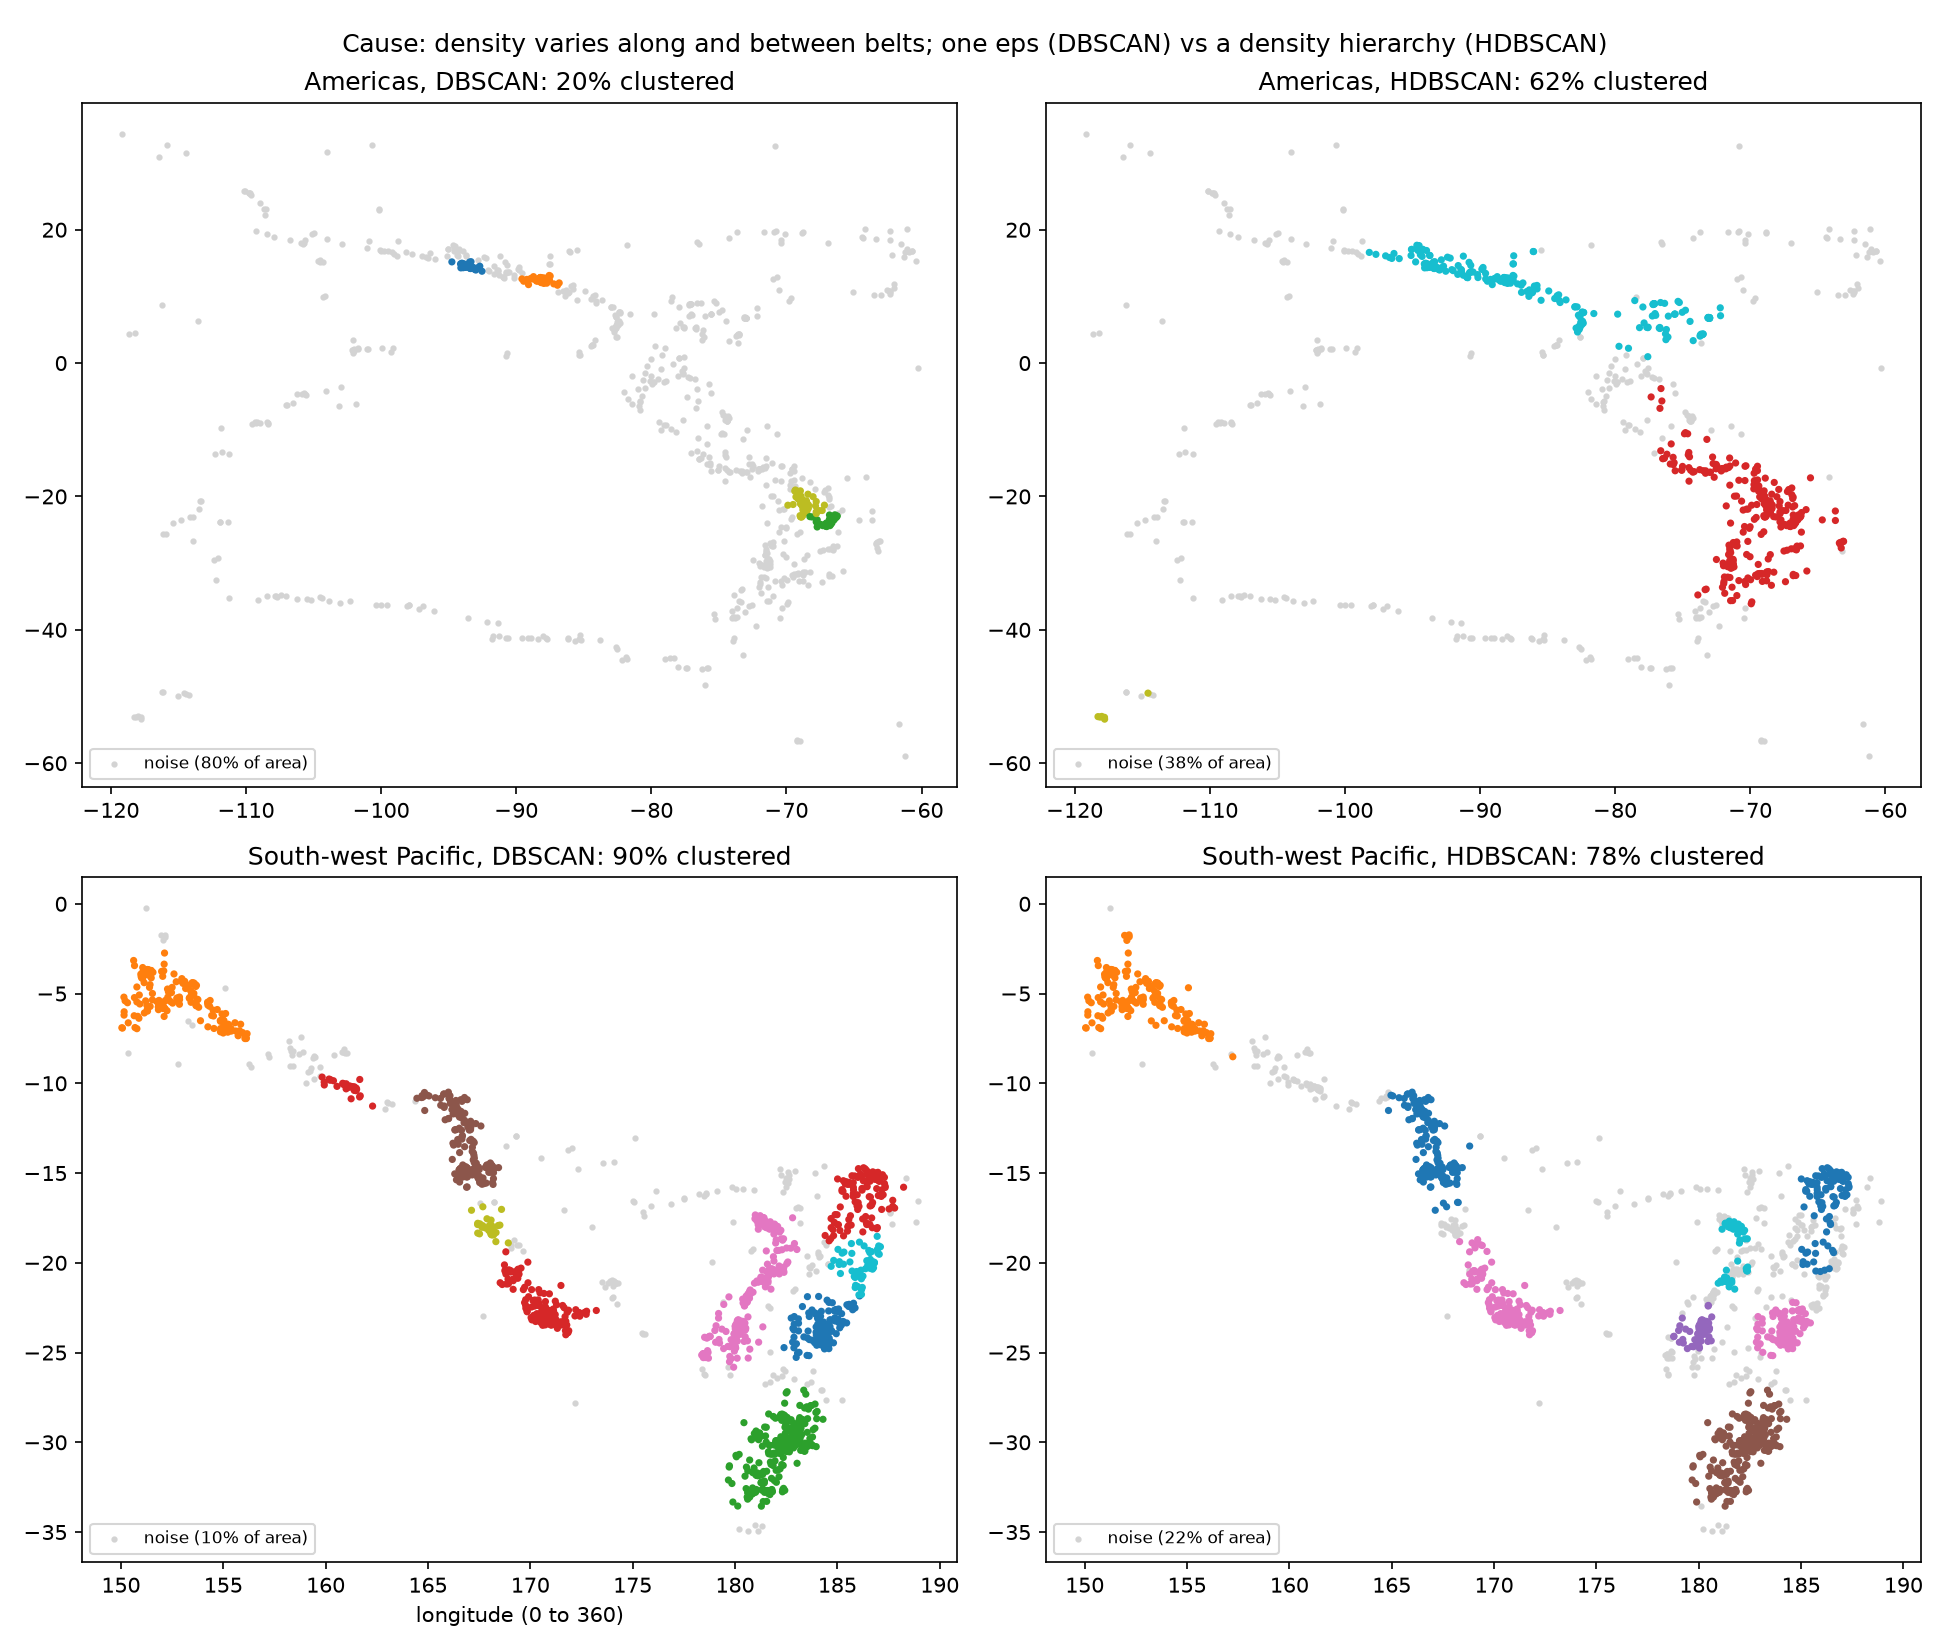
\includegraphics[width=0.85\textwidth]{eq_case_density_dbscan_vs_hdbscan}
\caption{D2, DBSCAN ($\varepsilon=101.8$\,km) against HDBSCAN in a sparse region (top, the Americas)
and a dense one (bottom, the south-west Pacific); grey points are noise. Success of HDBSCAN on the sparse
belts, at the cost of trimming the dense ones. Cause: density varies along and between belts.}
\label{fig:density}
\end{figure}
\todo{Ky + Hoang Anh}{D3: Midtown vs outer boroughs; knee $\varepsilon$ vs silhouette-optimal $\varepsilon$.}

\subsubsection{High dimensions}\label{sec:dims}
\owner{Ky (D4), Lam (D5)}
\todo{Ky}{D4: crossover between 3 and 4 PCA dimensions (Ablation D).}
\todo{Lam}{D5: DBSCAN ARI 0.033; HDBSCAN labels 71\% of points noise.}

\subsubsection{No gaps between groups}\label{sec:nogaps}
\owner{Wei Yew (D8)}
% Sources: weiyew/sc4020-hdb/results/comparison.csv, kmeans_k_sweep.csv, screening.csv.
D8 is one continuous mass: flats come in every combination of size, lease, storey and price, with no empty
space between groups. Table~\ref{tab:cmp_d2d8} shows what each method does with it. K-means still finds a
weak partition, four market segments (newer mid-size, older small, large older, newer high-floor), with a
silhouette of 0.317 against 0.218 on shuffled columns. That ratio of 1.45 is modest, but it is the only
result on D8 that beats its fake data. Density methods have no sparse region to cut along. The DBSCAN
setting chosen by the rule puts 97.1\% of sales in one cluster, and HDBSCAN finds one core holding 68.6\%
of sales plus a compact block of new 3-room flats, and calls 28.5\% noise. Both score below the same
setting on shuffled columns (0.239 against 0.330, and 0.160 against 0.593). On shuffled columns HDBSCAN calls
94.0\% of sales noise and keeps two small, well-separated clusters, which the silhouette rewards. On data
with no gaps, a density method has nothing to find, and the selection rule
cannot tell.

\begin{figure}[h]\centering
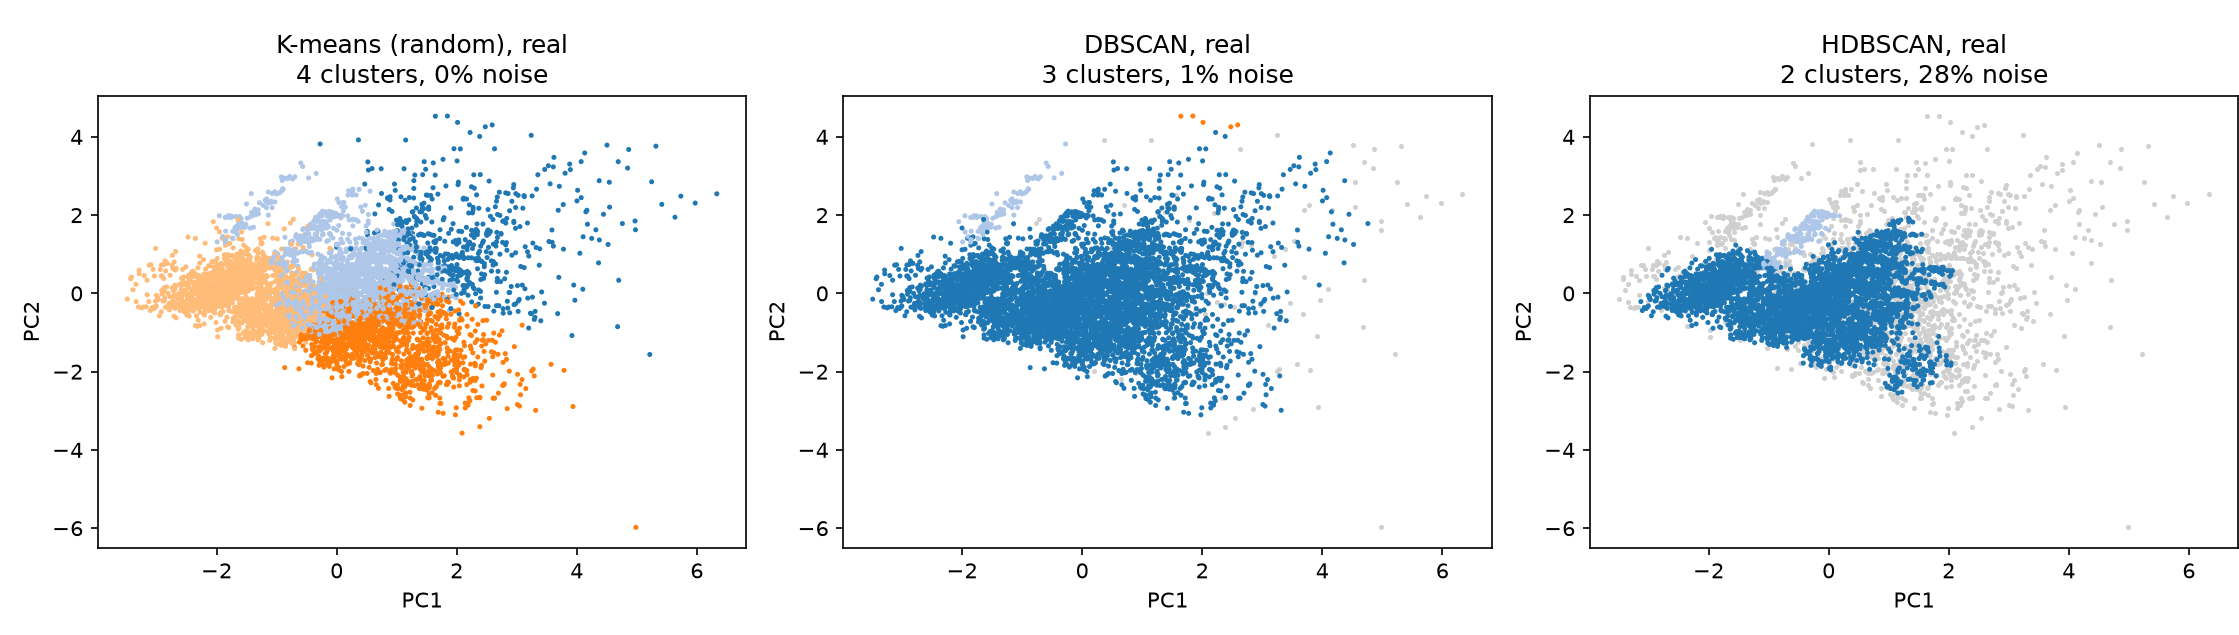
\includegraphics[width=0.95\textwidth]{hdb_comparison}
% Three of the six panels of weiyew/sc4020-hdb/figures/comparison.png (recorded data), cropped side by side.
\caption{D8 at the chosen settings on recorded data, drawn on the first two principal components
(6{,}000 sales; grey: noise). K-means cuts the mass into four segments; DBSCAN and HDBSCAN return one dominant cluster. Cause:
no gaps between groups.}
\label{fig:hdb_cmp}
\end{figure}

\subsubsection{Silhouette versus ground truth}\label{sec:silhouette}
\owner{All}
\todo{All}{One paragraph, one line per dataset:
D4 best silhouette (HDBSCAN) has the worst ARI, rank correlation $-0.80$ (Ky);
D6 DBSCAN silhouette 0.42 vs K-Means++ 0.28, ARI 0.31 vs 0.90 (Lam);
D7 K-Means top silhouette 0.343, GMM best ARI 0.774 vs 0.654 (Hoang Anh);
D8 unscaled K-means silhouette 0.540 from price bands, against 0.317 standardised (Wei Yew, written in
Ablation~C); D2 K-means silhouette flat at 0.516 to 0.532 for every $K$ from 4 to 12, so it cannot choose
$K$ (Wei Yew, \nolinkurl{weiyew/sc4020-earthquake/results/kmeans_k_selection.csv});
D5 HDBSCAN top silhouette with 71\% noise (Lam).}

\begin{figure}[h]\centering
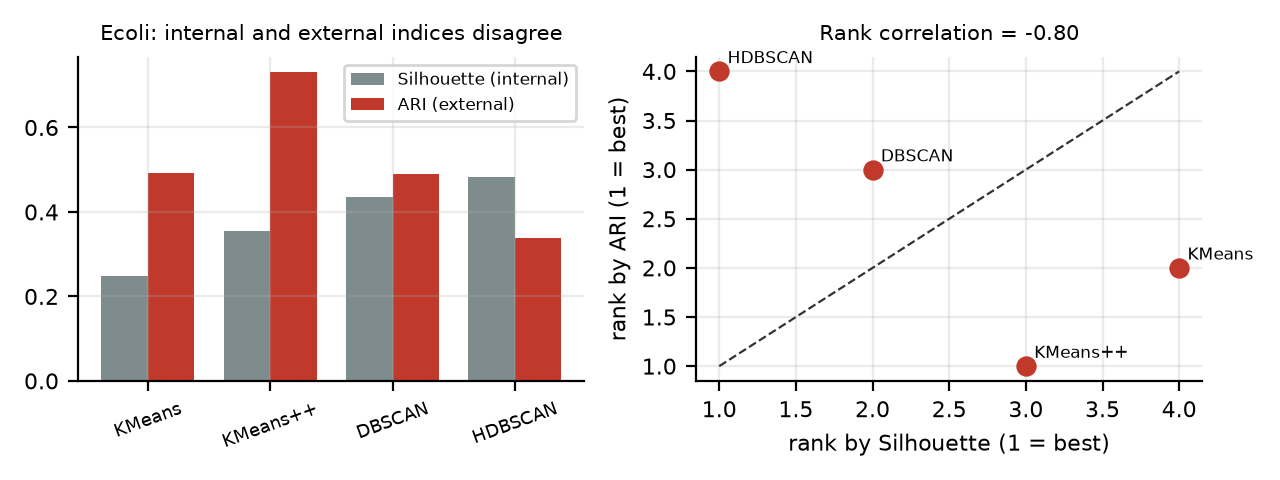
\includegraphics[width=0.72\textwidth]{f8_metric_disagreement}
\caption{\todo{Ky}{existing figure; extend to D5--D8 or make one panel per dataset.}}
\label{fig:silhouette}
\end{figure}

\subsection{Ablation studies}\label{sec:ablation}
\owner{Ky, Wei Yew}

% Rubric: "ablation study of the key components". One change at a time, everything else fixed.

\subsubsection{A: Initialisation (K-Means vs K-Means++)}
\todo{Ky}{Port Ablation A (30 seeds, D3/D4). Add ARI mean $\pm$ s.d.\ over the 30 seeds:
the 0.24 ARI claim currently rests on seed 42 only.}
\todo{Wei Yew}{D2: worst single-start run 18.8\% (random) vs 11.5\% (K-Means++) above the best.
D8: no difference, all 40 runs within 0.009\% of the best.}

\subsubsection{B: Distance on geographic coordinates}
\todo{Wei Yew}{Flat degrees vs sphere on D2: 92 close pairs straddle the $180^\circ$ line; sphere keeps
92 (K-means), 86 (DBSCAN), 79 (HDBSCAN) together, flat degrees 0. K-means silhouette 0.528
$\to$ 0.404. Source: \nolinkurl{weiyew/sc4020-earthquake/notebooks/ablation.ipynb}, Sec.~2.}
\decide{Ky's projected-km pipeline has the same $\pm180^\circ$ cut. Rerun D3 on the sphere,
or state that city scale makes it irrelevant.}

\subsubsection{C: Feature scaling}
\todo{Ky}{D4: standardisation lifts K-Means++ ARI 0.497 $\to$ 0.731; DBSCAN unaffected once
$\varepsilon$ is re-tuned.}
\todo{Wei Yew}{D8: raw units give price bands (silhouette 0.540, ARI 0.261 vs standardised).}

\subsubsection{D: Dimensionality}
\todo{Ky}{Port Ablation D. Call it PCA dimension; ``intrinsic dimensionality'' overclaims.}
\begin{figure}[h]\centering
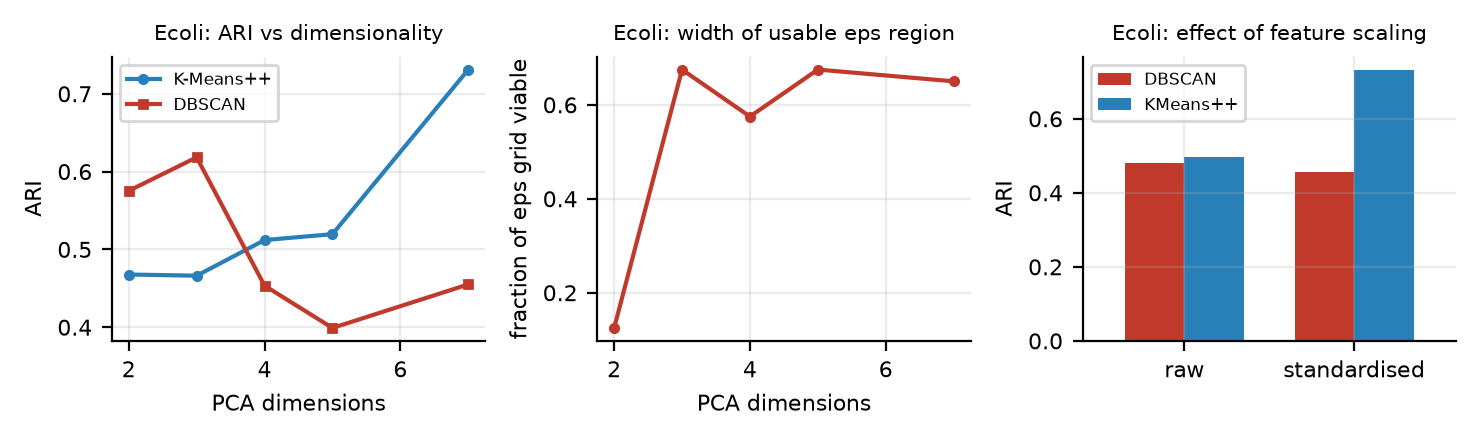
\includegraphics[width=\textwidth]{f7_ablations}
\caption{\todo{Ky}{existing figure (Ablations C and D on D4).}}
\label{fig:abl}
\end{figure}

\subsubsection{E: Values recorded in steps}
\todo{Wei Yew}{D8 storey bands: with a 50\% largest-cluster cap, 27 of 27 DBSCAN and 6 of 7 HDBSCAN
clusters are single storey bands; jittering within the band removes them.}

\subsubsection{F: Data subsets}
\todo{Wei Yew}{D2: magnitude 5.0+ behaves like a random subset of equal size; half-year vs
full-year HDBSCAN ARI 0.41--0.54.}

\subsection{Improvements to the methods}\label{sec:improve}
\owner{All}

% Rubric: "discuss or implement possible solutions to improve the methods".
% Each row: a failure we observed, its cause, the fix we implemented, and the measured effect.

\begin{table}[h]\centering\small
\caption{Implemented improvements. Each fix targets a failure observed in Section~\ref{sec:comparison}.}
\label{tab:improve}
\resizebox{\textwidth}{!}{\begin{tabular}{llllll}
\toprule
\textbf{Failure} & \textbf{Cause} & \textbf{Fix} & \textbf{Data} & \textbf{Before $\to$ after} & \textbf{Owner} \\
\midrule
Clusters split at $180^\circ$ & flat lat/lon & surface distance & D2 & 0 $\to$ 92 of 92 pairs kept & Wei Yew \\
Poor local optimum & random seeding & K-Means++ & D4 & ARI 0.493 $\to$ 0.731 & Ky \\
Sparse belts lost & one global $\varepsilon$ & HDBSCAN & D2 & Americas kept 20\% $\to$ 62\% & Wei Yew \\
One feature dominates & unequal scales & standardisation & D4 & ARI 0.497 $\to$ 0.731 & Ky \\
Clusters are storey bands & recorded steps & jitter within step & D8 & 27 of 27 band clusters $\to$ none & Wei Yew \\
Curved clusters cut & convex assumption & spectral clustering & D1 & ARI 0.481 $\to$ 1.000 & Lam \\
Degenerate $k$ chosen & silhouette alone & constraints + fake-data check & D2, D3 & \todo{Ky}{?} & Ky, Wei Yew \\
\bottomrule
\end{tabular}}
\end{table}

\todo{All}{One short paragraph per row: why the fix works, and its cost.}
\todo{All}{Proposed but not implemented: e.g.\ ground truth for D2 from plate-boundary maps;
OPTICS; approximate spectral clustering for large $n$.}

\subsection{Runtime and scalability}\label{sec:runtime}
\owner{Wei Yew, Lam}

\todo{Wei Yew}{D8, all 234{,}294 sales: K-means under 0.06\,s; HDBSCAN 212\,s; DBSCAN not run
(neighbour lists need about 6\,GB). Plot runtime against $n$ (\nolinkurl{weiyew/sc4020-hdb/experiments/scalability.py}).}
% Lam: lam/results/fashion_mnist_results.csv (fit_seconds; single fit at the chosen parameters, tuning excluded)
D5 was sampled down from 70{,}000 to 3{,}000 images because three methods scale badly with $n$ in
50 dimensions. Spectral clustering needs an $n\times n$ affinity matrix: dense, at $n=70{,}000$ it
takes about 39\,GB in double precision, and the eigenvector step grows faster than linearly even with
a sparse graph. DBSCAN and HDBSCAN rely on neighbour queries, and in 50 dimensions spatial indexes
prune little, so these queries approach the $O(n^2)$ brute-force cost. On the 3{,}000-point sample
one fit takes 0.011\,s for DBSCAN, 0.079\,s for K-Means++, 0.18\,s for Spectral, 0.30\,s for HDBSCAN
and 2.80\,s for GMM. GMM is the slowest here: with full covariances each EM step costs
$O(nkd^2)$ with $d=50$. These times exclude parameter search, which refits DBSCAN 15 times and
HDBSCAN 6 times.
\todo{Ky}{Existing Fig.~9 runtime at $n\leq23{,}412$, if kept.}

\begin{figure}[h]\centering
\figtodo{Wei Yew}{runtime vs number of sales, log--log, one line per method}
\caption{\todo{Wei Yew}{caption}}
\label{fig:runtime}
\end{figure}

\subsection{Success and failure cases}\label{sec:cases}
\owner{each owner: one figure per case, with the cause named in the caption}

% Rubric: "illustrate and discuss the successful cases and failure cases", "good visualizations".

\subsubsection{Successes}
\paragraph{HDBSCAN on D2: belts of varying density.} Shown in Figure~\ref{fig:density}. HDBSCAN keeps
the sparse belts of the Americas (62\% of earthquakes clustered, against 20\% for DBSCAN) as long
clusters that follow the plate boundary. It succeeds because its density threshold adapts to each
cluster, the property D2 needs most.
\habegin
% Source: hoanganh/comparison/results/report_d6_d7.csv; figure from hoanganh/comparison/run_report_tables.py.
\paragraph{GMM on D7: classes of unequal spread.} \hatag{} Shown in Figure~\ref{fig:bc_cases}. GMM matches the
diagnosis best of all methods (ARI 0.774). K-means places its boundary too far into the wide malignant
class (ARI 0.654); the full covariance of each GMM component lets the boundary follow the compact benign
class. Cause of success: the model allows clusters of different spread.
\haend
\todo{Lam}{DBSCAN / Spectral on D1.}
\todo{Ky}{K-Means++ on D4: compact classes in 7 dimensions.}
% Sources: weiyew/sc4020-hdb/results/ablation_features.csv, ablation_flat_design_clusters.csv
% (variant "floor area and lease only").
\paragraph{HDBSCAN on D8, floor area and lease only: flat designs.} This feature set was chosen after
seeing the main results, so we present it as an ablation finding and a sanity check, not as a tuned
setting. Dropped to two features, D8 does contain dense spots: standard flat designs, built to fixed
plans in particular years. HDBSCAN finds 14 clusters (43.2\% noise), and 13 of them are at least 97\% one
flat type (Figure~\ref{fig:flat_designs}); in the median cluster one flat model accounts for
83\% of sales. A simple grouping by flat
model and lease would give similar groups, which is the point: the method recovers a structure we can
name. ARI against flat type is still only 0.127, because each type is split into several designs and
the noise counts as a cluster. A low ARI here reflects a finer partition than the labels, not a failure.

\begin{figure}[h]\centering
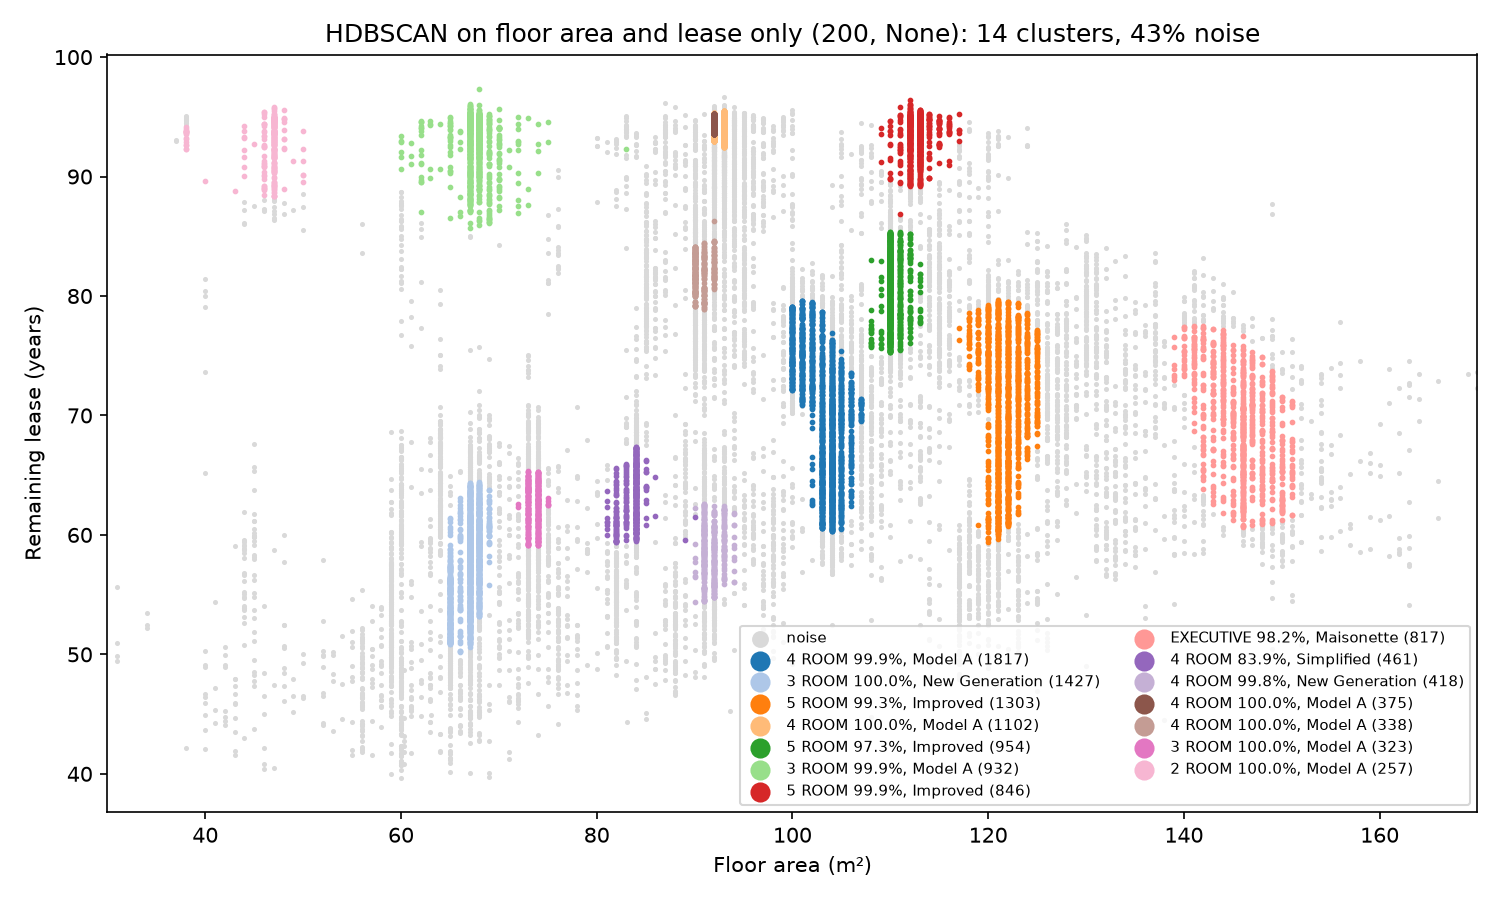
\includegraphics[width=0.8\textwidth]{hdb_success_flat_designs}
\caption{D8, success of HDBSCAN on floor area and remaining lease only (\texttt{min\_cluster\_size}~200;
grey: noise). Each cluster is one standard flat design; the legend gives its main flat type and model.
Cause of success: fixed building plans create real dense spots in these two features.}
\label{fig:flat_designs}
\end{figure}

\subsubsection{Failures}
\paragraph{K-Means++ on D2: unrelated belts merged.} Shown in Figure~\ref{fig:kmeans_belts}. One
cluster joins five belts whose centres are 2{,}932 to 11{,}449\,km apart, from Iceland to the
Mid-Indian Ridge. Cause: cluster shape. Compact regions cannot follow long belts.
\paragraph{Density methods on D8: one mass, or storey bands.} Shown in Figures~\ref{fig:hdb_cmp}
and~\ref{fig:abl_ties}. At the chosen settings DBSCAN puts 97.1\% of sales in one cluster. Under a cap on
the largest cluster, the clusters become single storey bands. Causes: no gaps between groups, and values
recorded in steps.
\habegin
\paragraph{DBSCAN on D7: half the data discarded.} \hatag{} Shown in Figure~\ref{fig:bc_cases}. The least noisy
two-cluster setting keeps the dense benign core as one cluster, finds a second cluster of 14 malignant tumours and
labels 55.5\% of tumours noise, including 183 of the 212 malignant ones. Its silhouette (0.356) is higher than that
of GMM or K-means, and its ARI is 0.222. Causes: 30 dimensions, and one class much sparser than the other.

\begin{figure}[h]\centering
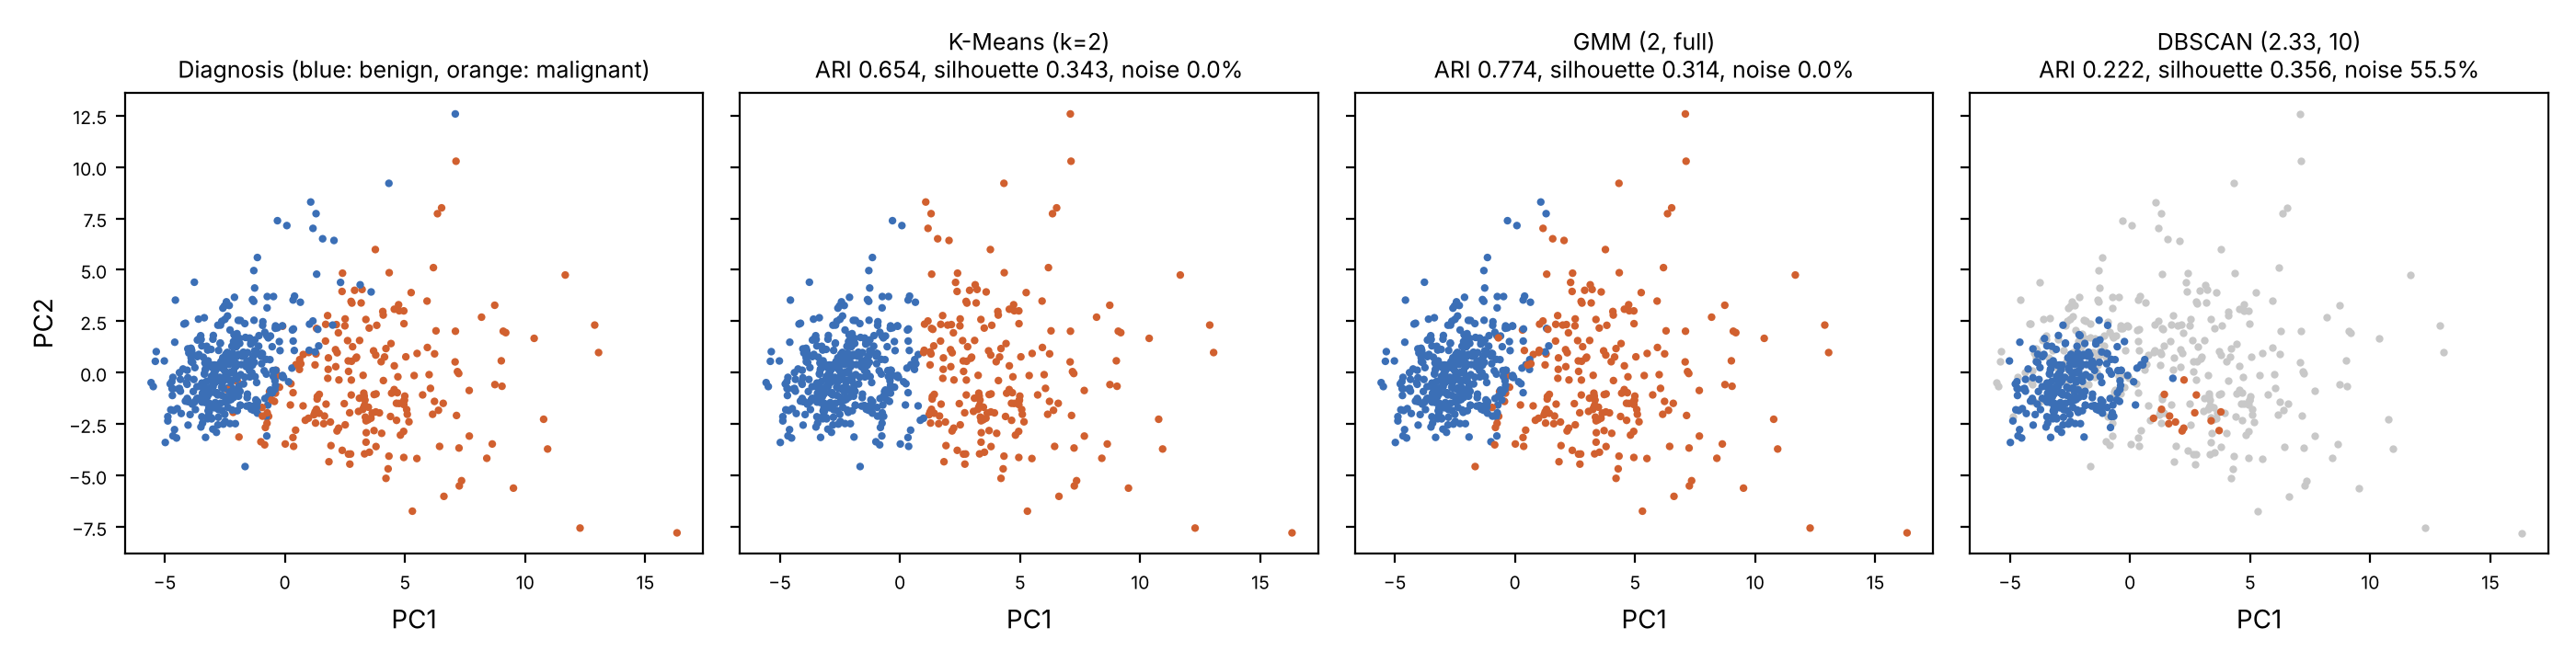
\includegraphics[width=\textwidth]{bc_cases}
\caption{\hatag D7 on its first two principal components (grey: noise; each cluster takes the colour
of its majority class). Success of GMM against K-means: the boundary follows the compact benign class.
Failure of DBSCAN: only the dense benign core is clustered. Causes: classes of unequal spread, and no
density contrast in 30 dimensions.}
\label{fig:bc_cases}
\end{figure}
\haend
\todo{Lam}{DBSCAN on D5.}
\todo{Ky}{HDBSCAN on D4: 37\% noise removes rare classes.}

\begin{figure}[h]\centering
\figtodo{All}{success/failure panel grid: one panel per case above}
\caption{\todo{All}{caption naming the cause of each case}}
\label{fig:cases}
\end{figure}

\subsection{Key factors and practical guidance}\label{sec:factors}
\owner{Ky}

% Rubric: "discuss the key factors that affect the performance".

% [Ky]: ranked by how much each factor changed the outcome; every number is quoted from the section cited.
\paragraph{Key factors.} Ordered by the size of their effect in our experiments:
\begin{enumerate}\itemsep1pt
\item \textbf{Cluster shape against the method's assumption.} On D1 K-Means++ reaches ARI 0.481 and
DBSCAN 0.98; on D2 K-means joins belts thousands of kilometres apart (Section~\ref{sec:shape}). No
parameter setting repairs a wrong assumption about shape.
\item \textbf{Gaps between groups.} Density methods need empty space between clusters. Where there is
none they return one dominant cluster: 97.1\% of sales on D8, 96.1\% of pickups on D3 and 97\% of proteins
on D4 at the settings chosen without labels (Sections~\ref{sec:nogaps} and \ref{sec:density}).
\item \textbf{Dimensionality.} On D4 the ranking of DBSCAN and K-Means++ reverses between 3 and 4
principal components (Ablation~D); on D5, with 50 dimensions, DBSCAN reaches ARI 0.03 and HDBSCAN
calls 71\% of points noise (Section~\ref{sec:dims}).
\item \textbf{Uneven density.} One DBSCAN radius clusters 90\% of the dense south-west Pacific but 20\%
of the Americas on D2; HDBSCAN raises the Americas to 62\% (Section~\ref{sec:density}).
\item \textbf{Parameter choice without labels.} On D4 the rule's DBSCAN setting scores ARI 0.039 against
0.489 at the best setting; on D3 the knee and the silhouette-best radius differ threefold and give 13 and
2 clusters (Table~\ref{tab:cmp_d3d4}).
\item \textbf{Feature scaling.} Standardising D4 raises K-Means++ ARI from 0.497 to 0.731; on D8, raw
units turn K-means into price bands (Ablation~C).
\item \textbf{Values recorded in steps.} On D8, 107 of 124 HDBSCAN clusters are single storey bands on
the recorded data and none on jittered data (Ablation~E).
\item \textbf{Initialisation.} Over 30 seeds K-Means++ raises mean ARI on D4 from 0.485 to 0.561, and on
D2 it cuts the mean gap to the best inertia from 10.9\% to 4.8\%; on D3 and D8 it makes no difference to
the result (Ablation~A).
\item \textbf{Runtime.} It only matters at the size of D8, where HDBSCAN takes 212\,s and DBSCAN runs out
of memory (Section~\ref{sec:runtime}).
\end{enumerate}
% [Wei Yew]: evidence for the two guidance items handed to Ky.
% Fake-data check: D2 K=2 silhouette 0.544 vs 0.529 on shuffled coordinates (kmeans_k_selection.csv);
% D8 density methods below their null (comparison.csv). Recorded steps: D8 107 of 124 HDBSCAN clusters
% are single storey bands on recorded data, 0 of 23 on jittered data (hdbscan_grid.csv).
\paragraph{Practical guidance.}
\begin{enumerate}\itemsep1pt
\item \textbf{Choose by the structure of the data, not by a score.} Plot the data or a projection first.
If the groups are curved or long, no choice of $k$ will help K-means; if they are compact and touching,
or the data have more than a handful of dimensions, no choice of $\varepsilon$ will help DBSCAN.
\item \textbf{Do not pick settings by the silhouette alone.} It favours few, round clusters and settings
that call hard points noise. First restrict the search to what the analysis needs (a noise cap, a
minimum number of clusters), then compare within that range.
\item \textbf{Report the noise fraction and the largest cluster next to every silhouette.} A silhouette
computed after discarding 37\% of the points, or with 97\% in one cluster, says little.
\item \textbf{Compare every result against fake data.} Rerun the chosen setting on shuffled columns or
uniform points. It catches results with no real structure (D4 density methods, D8), though not results
with the wrong structure (D2).
\item \textbf{Check for values recorded in steps.} Tied values such as storey bands form dense spots that
density methods report as clusters; add jitter within each step and see whether the clusters remain.
\item \textbf{Standardise before K-means, and use K-means++ with several starts.} One K-means++ start is
not enough when the objective has many local optima (D2).
\item \textbf{Prefer a parameter whose unit means something, and measure distance correctly.} A radius
in kilometres can be checked by someone who knows the area; a $k$ cannot. Use distance on the sphere for
global coordinates (D2); a local projection is enough within a city (D3).
\end{enumerate}


\section{Conclusion}\label{sec:conclusion}
\owner{Ky}
\todo{Ky}{Summary of findings with numbers; answer the title question.}

\subsection*{Limitations}
\todo{All}{One line each: D2 has no ground truth; D8 has no location feature; oracle ARI on labelled
data is optimistic; datasets up to 50 dimensions.}

% Shared bibliography. Add entries in alphabetical order of key; cite with \cite{key}.
\begin{thebibliography}{99}\small\itemsep0pt
\bibitem{ankerst1999} M.~Ankerst, M.~M. Breunig, H.-P. Kriegel, and J.~Sander. OPTICS: Ordering points to identify the clustering structure. In \emph{Proc.\ ACM SIGMOD}, pp.~49--60, 1999.
\bibitem{arthur2007} D.~Arthur and S.~Vassilvitskii. k-means++: The advantages of careful seeding. In \emph{Proc.\ 18th ACM-SIAM SODA}, pp.~1027--1035, 2007.
\bibitem{beyer1999} K.~Beyer, J.~Goldstein, R.~Ramakrishnan, and U.~Shaft. When is ``nearest neighbor'' meaningful? In \emph{Proc.\ ICDT}, LNCS 1540, pp.~217--235, 1999.
\bibitem{calinski1974} T.~Cali\'nski and J.~Harabasz. A dendrite method for cluster analysis. \emph{Communications in Statistics}, 3(1):1--27, 1974.
\bibitem{campello2013} R.~J.~G.~B. Campello, D.~Moulavi, and J.~Sander. Density-based clustering based on hierarchical density estimates. In \emph{Proc.\ PAKDD}, LNCS 7819, pp.~160--172, 2013.
\bibitem{davies1979} D.~L. Davies and D.~W. Bouldin. A cluster separation measure. \emph{IEEE TPAMI}, 1(2):224--227, 1979.
\bibitem{dempster1977} A.~P. Dempster, N.~M. Laird, and D.~B. Rubin. Maximum likelihood from incomplete data via the EM algorithm. \emph{J.\ Royal Statistical Society B}, 39(1):1--38, 1977.
\bibitem{ester1996} M.~Ester, H.-P. Kriegel, J.~Sander, and X.~Xu. A density-based algorithm for discovering clusters in large spatial databases with noise. In \emph{Proc.\ KDD}, pp.~226--231, 1996.
\bibitem{hopkins1954} B.~Hopkins and J.~G. Skellam. A new method for determining the type of distribution of plant individuals. \emph{Annals of Botany}, 18(2):213--227, 1954.
\bibitem{horton1996} P.~Horton and K.~Nakai. A probabilistic classification system for predicting the cellular localization sites of proteins. In \emph{Proc.\ ISMB}, pp.~109--115, 1996.
\bibitem{hubert1985} L.~Hubert and P.~Arabie. Comparing partitions. \emph{Journal of Classification}, 2(1):193--218, 1985.
\bibitem{lloyd1982} S.~P. Lloyd. Least squares quantization in PCM. \emph{IEEE Trans.\ Information Theory}, 28(2):129--137, 1982.
\bibitem{luxburg2012} U.~von Luxburg, R.~C. Williamson, and I.~Guyon. Clustering: Science or art? In \emph{Proc.\ ICML Workshop on Unsupervised and Transfer Learning}, JMLR W\&CP 27:65--79, 2012.
\bibitem{moulavi2014} \ha{D.~Moulavi, P.~A. Jaskowiak, R.~J.~G.~B. Campello, A.~Zimek, and J.~Sander. Density-based clustering validation. In \emph{Proc.\ SIAM SDM}, pp.~839--847, 2014.}
\bibitem{ng2002} A.~Y. Ng, M.~I. Jordan, and Y.~Weiss. On spectral clustering: Analysis and an algorithm. In \emph{Advances in NIPS 14}, pp.~849--856, 2002.
\bibitem{pedregosa2011} F.~Pedregosa et al. Scikit-learn: Machine learning in Python. \emph{JMLR}, 12:2825--2830, 2011.
\bibitem{rousseeuw1987} P.~J. Rousseeuw. Silhouettes: A graphical aid to the interpretation and validation of cluster analysis. \emph{J.\ Computational and Applied Mathematics}, 20:53--65, 1987.
\bibitem{tibshirani2001} R.~Tibshirani, G.~Walther, and T.~Hastie. Estimating the number of clusters in a data set via the gap statistic. \emph{J.\ Royal Statistical Society B}, 63(2):411--423, 2001.
\bibitem{ward1963} J.~H. Ward. Hierarchical grouping to optimize an objective function. \emph{J.\ American Statistical Association}, 58(301):236--244, 1963.
\bibitem{xiao2017} H.~Xiao, K.~Rasul, and R.~Vollgraf. Fashion-MNIST: A novel image dataset for benchmarking machine learning algorithms. arXiv:1708.07747, 2017.
% ---- dataset sources: each owner adds theirs ----
\bibitem{usgs2017} U.S. Geological Survey, Earthquake Hazards Program. Advanced National Seismic System (ANSS) Comprehensive Catalog of Earthquake Events and Products, 2017. doi:10.5066/F7MS3QZH.
\bibitem{hdb2026} Housing \& Development Board. Resale flat prices based on registration date from Jan-2017 onwards; HDB Resale Price Index (1Q2009 = 100), Quarterly. data.gov.sg, accessed 14 September 2026, Singapore Open Data Licence v1.0.
\bibitem{aeberhard1991} \ha{S.~Aeberhard and M.~Forina. Wine. UCI Machine Learning Repository, 1991. doi:10.24432/C5PC7J.}
\bibitem{street1993} \ha{W.~N. Street, W.~H. Wolberg, and O.~L. Mangasarian. Nuclear feature extraction for breast tumor diagnosis. In \emph{Proc.\ SPIE 1905, Biomedical Image Processing and Biomedical Visualization}, pp.~861--870, 1993.}
\item[] \todo{Ky + Hoang Anh}{Uber source: FiveThirtyEight, Uber pickups in New York City (April 2014 file); agree which copy to cite.} \todo{Lam}{Mall.}
\end{thebibliography}

\end{document}
